\documentclass[12pt]{article}

\usepackage{amsmath,amsthm,amsfonts,amssymb,amsxtra}
\usepackage{pgf,tikz}
\usetikzlibrary{arrows}
\renewcommand{\theenumi}{(\alph{enumi})} 
\renewcommand{\labelenumi}{\theenumi}

\pagestyle{empty}
\setlength{\textwidth}{7in}
\setlength{\oddsidemargin}{-0.5in}
\setlength{\topmargin}{-1.0in}
\setlength{\textheight}{9.5in}

\newtheorem{problem}{Problem}

\begin{document}

\noindent{\large\bf MATH 141}\hfill{\large\bf Exam\#1.}\hfill{\large\bf
  Fall 2007}\hfill{\large\bf Page 1/7}\hrule

\bigskip
\begin{center}
  \begin{tabular}{|ll|}
    \hline & \cr
    {\bf Name: } & \makebox[12cm]{\hrulefill}\cr & \cr
    {\bf 4-digit code:} & \makebox[12cm]{\hrulefill}\cr & \cr
    \hline
  \end{tabular}
\end{center}
\begin{itemize}
\item Write your name and the last 4 digits of your SSN in the space provided above.
\item The test has seven (7) pages, including this one.
\item For multi-choice questions, you should circle the answer you
  select.  On the other problems, you should enter your answer in the
  box(es) provided.
\item You must show sufficient work to justify all answers unless
  otherwise stated in the problem.  Correct answers with inconsistent
  work may not be given credit.
\item Credit for each problem is given in parentheses at the right of
  the problem number.
\item No books, notes or calculators may be used on this test.
\end{itemize}
\hrule

\begin{center}
  \begin{tabular}{|c|c|c|}
    \hline
    &&\cr
    {\large\bf Page} & {\large\bf Max.~points} & {\large\bf Your points} \cr
    &&\cr
    \hline
    &&\cr
    {\Large 2} & \Large 20 & \cr
    &&\cr
    \hline
    &&\cr
    {\Large 3} & \Large 20 & \cr
    &&\cr
    \hline
    &&\cr
    {\Large 4} & \Large 30 & \cr
    &&\cr
    \hline
    &&\cr
    {\Large 5} & \Large 10 & \cr
    &&\cr
    \hline
    &&\cr
    {\Large 6} & \Large 10 & \cr
    &&\cr
    \hline
    &&\cr
    {\Large 7} & \Large 10 & \cr
    &&\cr
    \hline\hline
    &&\cr
    {\large\bf Total} & \Large 100 & \cr
    &&\cr
    \hline
  \end{tabular}
\end{center}
\newpage

%%%%%%%%%%%%%%%%%%%%%%%%%%%%%%%%%%%%% Page 1
\noindent{\large\bf MATH 141}\hfill{\large\bf Exam\#1.}\hfill{\large\bf
  Fall 2007}\hfill{\large\bf Page 2/7}\hrule

\bigskip
{\problem[20 pts] \em  Answer the following questions:}
\begin{enumerate} 
\item What is the domain of the following function? (justify your answer)
\begin{equation*}
f(x) = \frac{x}{\sqrt{x-2}}.
\end{equation*}
\begin{enumerate}
\item $x < 2$
\item $x \leq 2$
\item $x \geq 2$
\item $x > 2$
\item $x \neq 2$
\end{enumerate}
\vspace{4cm}
\hrule
\item Complete the following table (no explanations needed!)
\begin{equation*}
\begin{array}{||c||c|c|c|c|c||}
\hline x & \quad -2 \quad & \quad -1\quad & \quad 0\quad  & \quad 1\quad  & \quad 2\quad  \\
\hline f(x) & -1 & 2 & 0 & -2 & 1 \\
\hline g(x) & 2 & 0 & -1 & 2 & -1\\
\hline \hline & & & & & \\
 (f \circ g)(x) & & & & & \\ & & & & & \\
\hline \hline & & & & & \\
 (g \circ f)(x) & & & & & \\ & & & & & \\
\hline
\end{array}
\end{equation*}
\end{enumerate}
\newpage

%%%%%%%%%%%%%%%%%%%%%%%%%%%%%%%%%%%%% Page 2
\noindent{\large\bf MATH 141}\hfill{\large\bf Exam\#1.}\hfill{\large\bf
  Fall 2007}\hfill{\large\bf Page 3/7}\hrule

\bigskip
{\problem[10pts] \em Find the amplitude and period of}
\begin{equation*}
y = 3 \cos \big( 2x + \tfrac{\pi}{2} \big).
\end{equation*}
\vspace{6cm}
\begin{flushright}
  \begin{tikzpicture}
    \draw (-1.25cm,0.5cm) node {$\text{Amplitude} =$};
    \draw (0cm,0cm) rectangle (5cm,1.2cm);
    \draw (-1cm,2cm) node {$\text{period} =$};
    \draw (0cm,1.4cm) rectangle (5cm,2.6cm);
  \end{tikzpicture}
\end{flushright}
\hrule

{\problem[10 pts] \em Solve for $x$:}
\begin{equation*}
\log (3x) - 3 \log (x^{-1/3}) = \log 27.
\end{equation*}
\vspace{6cm}
\begin{flushright}
  \begin{tikzpicture}
    \draw (-1cm,0.5cm) node {$x =$};
    \draw (0cm,0cm) rectangle (5cm,1.2cm);
  \end{tikzpicture}
\end{flushright}
\newpage

%%%%%%%%%%%%%%%%%%%%%%%%%%%%%%%%%%%%% Page 3
\noindent{\large\bf MATH 141}\hfill{\large\bf Exam\#1.}\hfill{\large\bf
  Fall 2007}\hfill{\large\bf Page 4/7}\hrule

\bigskip
{\problem[30 pts] \em Compute the following limits:}

\bigskip
\noindent
\begin{tikzpicture}
\draw (4cm,14cm) node{
(a) $\displaystyle{\lim_{x \to 2} \frac{x^2-2x-8}{x^2-4}} = \mbox{}$ };
\draw (6cm,13.4cm) rectangle (11cm,14.6cm);
\draw (4cm, 7cm) node{
(b) $\displaystyle{\lim_{x \to \infty} \frac{x^2-2x-8}{x^2-4}} = \mbox{}$}; \draw (6.1cm,6.4cm) rectangle (11.1cm,7.6cm);
\draw (4cm, 0cm) node{
(c) $\displaystyle{\lim_{x \to \infty} \Big( 1 + \frac{5}{x} \Big)^{3x}} = \mbox{}$}; 
\draw (6cm,-0.6cm) rectangle (11cm,0.6cm);
\end{tikzpicture}
\newpage

%%%%%%%%%%%%%%%%%%%%%%%%%%%%%%%%%%%%% Page 4
\noindent{\large\bf MATH 141}\hfill{\large\bf Exam\#1.}\hfill{\large\bf
  Fall 2007}\hfill{\large\bf Page 5/7}\hrule

\bigskip
{\problem[10 pts] \em Recall the ``$\varepsilon$--$\delta$'' definition of limit:
\begin{center}
\begin{tikzpicture}
\draw (0.5\linewidth, 0cm) node[text justified, text width=0.5\linewidth, draw, rounded corners] {
We say $\displaystyle{\lim_{x\to a}} f(x) = b$ if for all $\varepsilon > 0$ there exists $\delta >0$ such that $\lvert x - a \rvert < \delta$ implies $\lvert f(x) - b \rvert < \varepsilon$.};
\end{tikzpicture}
\end{center}
Use this definition to prove that $\displaystyle{\lim_{x \to 4} x^2-2x = 8}$.}
\newpage

%%%%%%%%%%%%%%%%%%%%%%%%%%%%%%%%%%%%% Page 5
\noindent{\large\bf MATH 141}\hfill{\large\bf Exam\#1.}\hfill{\large\bf
  Fall 2007}\hfill{\large\bf Page 6/7}\hrule

\bigskip
{\problem[10 pts] \em Find the value of the constant $k$ for which the following function is continuous everywhere:}
\begin{equation*}
f(x) = \begin{cases}
2k^2x^3 &\text{if }x<2, \\
x+32k-18 &\text{if }x \geq 2.
\end{cases}
\end{equation*}
\vspace{16cm}
\begin{flushright}
  \begin{tikzpicture}
    \draw (-1cm,0.5cm) node {$k =$};
    \draw (0cm,0cm) rectangle (5cm,1.2cm);
  \end{tikzpicture}
\end{flushright}
\newpage

%%%%%%%%%%%%%%%%%%%%%%%%%%%%%%%%%%%%% Page 6
\noindent{\large\bf MATH 141}\hfill{\large\bf Exam\#1.}\hfill{\large\bf
  Fall 2007}\hfill{\large\bf Page 7/7}\hrule

\bigskip
{\problem[10 pts] Sketch the curve by eliminating the parameter (i.e.~try to write $y=f(x)$), and indicate the direction of increasing $t$}
\begin{equation*}
x=\sqrt{t},\quad y=2t+4.
\end{equation*}
\begin{center}
\begin{tikzpicture}
\clip (0cm, 0cm) rectangle (10cm,10cm);
\begin{scope}[xshift=5cm, yshift=5cm]
\draw[gray, very thin, step=0.5cm] (-4.4cm,-4.4cm) grid (4.4cm, 4.4cm);
\draw[<->, very thick] (0cm, -5cm) -- (0cm, 5cm);
\draw[<->, very thick] (-5cm, 0cm) -- (5cm, 0cm);
\end{scope}
\end{tikzpicture}
\end{center}

\end{document}